\documentclass[review,3p]{elsarticle}

\usepackage{lineno,hyperref}
\modulolinenumbers[5]
\usepackage{subcaption}             % used in subtable
\usepackage{amsmath,amsfonts,amsthm}            % for subequations

\usepackage{mathtools,amssymb}          % for \leqslant
\newcommand{\ddn}[2]{\frac{\mathrm{d}}{\mathrm{d}#1}#2}
\newcommand{\ddt}{\frac{\mathrm{d}}{\mathrm{d}t}}


\usepackage{upgreek}
\usepackage[dvipsnames]{xcolor}
\usepackage{soul}
\usepackage{multirow}

\usepackage{array}
\newcolumntype{C}[1]{>{\centering\let\newline\\\arraybackslash\hspace{0pt}}m{#1}} 
\newcolumntype{L}[1]{>{\raggedright\let\newline\\\arraybackslash\hspace{0pt}}m{#1}} 
\newcolumntype{R}[1]{>{\raggedleft\let\newline\\\arraybackslash\hspace{0pt}}m{#1}} 

\usepackage{booktabs}       % http://ctan.org/pkg/booktabs

\newcommand{\tabitem}{~~\llap{\textbullet}~~}           % for items inside a table
\usepackage{makecell}       % used inside a table
\usepackage{pbox}           % for weak form 3
\usepackage{empheq}
\newcommand*\widefbox[1]{\fbox{\hspace{2em}#1\hspace{2em}}}


\usepackage{colortbl}
\usepackage{esvect}
\usepackage{spreadtab}
\usepackage{numprint}
\usepackage{xstring}
\renewcommand*{\thefootnote}{\fnsymbol{footnote}}
\usepackage[symbol]{footmisc}

\usepackage{siunitx}

\makeatletter       % for rom in deal.ii symbol
\newcommand*{\rom}[1]{\expandafter\@slowromancap\romannumeral #1@}
\makeatother

\usepackage{enumitem}

\usepackage{cleveref}
\crefformat{section}{\S#2#1#3} % see manual of cleveref, section 8.2.1
\crefformat{subsection}{\S#2#1#3}
\crefformat{subsubsection}{\S#2#1#3}

\captionsetup[figure]{labelfont={bf},name={Fig.},labelsep=period}
\captionsetup[table]{labelfont={bf},name={Table},labelsep=space,justification=justified,singlelinecheck=false}      % the last two commands for left-align the caption

\usepackage[labelformat=simple]{subcaption}	        	% order of subfigure with brackets
\renewcommand\thesubfigure{(\alph{subfigure})}
\renewcommand\thesubtable{(\alph{subtable})}


\usepackage{graphicx}
\usepackage{wrapfig}
\usepackage{lipsum}

\usepackage{pgfplots}       % for tikzpicture

\pdfsuppresswarningpagegroup=1      % eliminate warning 'multiple pdfs with page group included in a single page'

\usepackage[ruled,linesnumbered]{algorithm2e}		% for algorithm






\begin{document}

\begin{frontmatter}

\title{Balancing truncation and round-off errors in practical FEM: one-dimensional analysis}

 \author[1]{Jie Liu\corref{cor1}}
 \ead{j.liu-5@tudelft.nl}
 \author[1]{Matthias M\"oller}
 \ead{m.moller@tudelft.nl}
 \author[1]{Henk M. Schuttelaars}
 \ead{h.m.schuttelaars@tudelft.nl}
 
 \address[1]{Delft Institute of Applied Mathematics\\ Delft University of Technology\\ Van Mourik Broekmanweg 6, 2628 XE Delft, The Netherlands}
\cortext[cor1]{Corresponding author}

\begin{abstract}
In finite element methods (FEMs), the accuracy of the solution cannot increase indefinitely because the round-off error increases when the number of degrees of freedom (DoFs) is large enough. This means that the accuracy that can be reached is limited. A priori information of the highest attainable accuracy is therefore of great interest.   
In this paper, we devise an innovative method to obtain the highest attainable accuracy.
In this method, the truncation error is extrapolated when it converges at the analytical rate, for which only a few primary $h$-refinements are required, and the bound of the round-off error is provided through extensive numerical experiments. The highest attainable accuracy is obtained by minimizing the sum of these two types of errors.
We validate this method using a one-dimensional Helmholtz equation in space. 
It shows that the highest attainable accuracy can be accurately predicted, and the CPU time required is much less compared with that using the successive $h$-refinement. 
\end{abstract}

\begin{keyword}
Finite Element Method (FEM), error estimation, optimal number of degrees of freedom, $hp$-refinement strategy.
\end{keyword}

\end{frontmatter}

\section{Introduction}

Many problems in engineering sciences and industry are modelled mathematically by initial-boundary value problems comprising systems of coupled, nonlinear partial and/or ordinary differential equations. These problems often consider complex geometries, with initial and/or boundary conditions that depend on measured data \cite{Kumar2016}. 
In some applications, not only the solution, but also its derivatives are of interest \cite{Kumar2016,carey1982derivative}.
For many problems of practical interest, analytical or semi-analytical solutions are not available, and hence one has to resort to numerical solution methods, such as the finite difference, finite volume, and finite element methods. The latter will be adopted throughout this paper and applied to one-dimensional boundary value problems.

The accuracy of the numerically obtained solution is influenced by many sources of errors \cite{ferziger2012computational}: firstly, errors in the set-up of the models, such as the simplification of the domain and governing equations and the approximation of the initial and boundary conditions; next, truncation errors due to the discretization of the computational domain and the use of basis functions for the function spaces defined on it; then, the iteration error resulting from the artificially controlled tolerance of iterative solvers; finally, the round-off error due to the adoption of finite-precision computer arithmetics, rather than exact arithmetics.
One tacitly assumes that most errors are well-balanced and/or negligibly small.
In particular, the round-off error is often ignored based on the argument that it will be `sufficiently small' if just IEEE-754 double-precision floating-point arithmetics \cite{zuras2008ieee} are adopted.
In this paper, the focus is on the overall discretization error due to truncation and round-off. In particular, we will show that the latter might very well have a significant influence on the overall accuracy and propose a practical strategy to balance both error contributors.

The discretization error strongly depends on the number of degrees of freedom (``DoFs"), denoted by $N_h^{(p)}$, which is a function of the mesh width $h$ and the approximation order $p$. The truncation error, denoted by ${E}_{\rm {T}}$, dominates the discretization error only when $N_h^{(p)}$ is not too large, and it decreases with increasing mesh resolution and element degree as it can be expected from finite element theory \cite{gockenbach2006understanding}. Based on this, the commonly used approaches to reduce the truncation error are to reduce the mesh width ($h$-refinement), increase the approximation order ($p$-refinement), or apply both strategies simultaneously ($hp$-refinement) \cite{guo1986hp}. 
The round-off error, denoted by ${E}_{\rm R}$, is, however, only negligible for moderately small values of $N_h^{(p)}$ and dominates the overall discretization error if more and more DoFs are employed \cite{Babuska2018Roundoff}. 
Consequently, for a particular approximation order $p$, by performing $h$-refinement, the best accuracy is obtained at the break-even point where the discretization error is the smallest. We denote the highest accuracy by ${E}_{\rm {min}}^{(p)}$ and the optimal number of DoFs by $N_{\rm opt}^{(p)}$.

While $N_{\rm opt}^{(p)}$ is typically impractically large if low(est)-order approximations are used, it can be very small if high-order approximations are adopted, which are nowadays becoming more and more popular, and make the results more prone to be polluted by round-off errors.
Despite this alarming observation, to the authors’ best knowledge, only very few publications address the impact of accumulated round-off errors on the overall accuracy of the final solution \cite{ling1984numerical,mou2017example} or take them into account explicitly in the error-estimation procedure {\cite{ainsworth1992procedure,kelly1983posteriori}}.
The general rule of thumb is still to perform as many $h$-refinements as possible considering the available computer hardware.

The aim of this paper is to systematically analyze the influence of the round-off error on the discretization error, for the solution, and its first and second derivative, and propose a practical approach for obtaining ${E}_{\rm {min}}^{(p)}$.
The scope is restricted to one-dimensional model problems, i.e. Poisson, diffusion and Helmholtz equations, for which both the standard finite element method (FEM) and the mixed FEM\cite{boffi2013mixed} are considered.
To assess the general applicability of the aforementioned approach, the following factors are investigated: the element degree over a wide range, first and second derivative of the solution, type of boundary conditions and method of implementing them, choice and configuration of the linear system solver, order of magnitude of the solution and its derivatives, and equation type.

The paper is organized as follows. The model problem, finite element formulation and numerical implementation are described in Section \ref{section_model_problem_FEM_formulation_numerical_implementation}. The general behavior of the discretization error and the approach to predict ${E}_{\rm {min}}^{(p)}$ are discussed in Section \ref{section_behaviour_discretization_error}. Numerical results for determining the offset of the round-off error are shown in Section \ref{section_error_constants}. The algorithm for realizing the approach is put forward in Section \ref{section_algorithm}, followed by its validation by a Helmholtz problem in Section \ref{section_validation}. The conclusions are drawn in Section \ref{paragraph on conclusion}.


\section{Model problem, finite element formulation and numerical implementation}	\label{section_model_problem_FEM_formulation_numerical_implementation}

\subsection{Model problem}

Consider the following one-dimensional second-order differential equation:
\begin{equation}
  -\left(d(x) u_x \right)_x + r(x)u(x) = f(x),\qquad x \in I = (0,1),	\label{1D_general_Helmholtz_equation}
\end{equation}
with $u$ denoting the unknown variable, which can either be real or complex, $f(x) \in L^2 (I)$ a prescribed right-hand side, and $d(x)$ and $r(x)$ continuous coefficient functions.
By choosing $d(x)=1$ and $r(x)=0$, Eq. (\ref{1D_general_Helmholtz_equation}) reduces to the Poisson equation; for $d(x)>0$ and not constant, when $r(x)=0$, the diffusion equation is found, and when $r(x) \neq 0$, we obtain the Helmholtz equation. 
The boundary conditions are $u(x)=g(x)$ on $\Gamma_D$ and $d(x)u_x=h(x)$ on $\Gamma_N$. Here, $\Gamma_D$ and $\Gamma_N$ are the boundaries where Dirichlet and Neumann boundary conditions are imposed, respectively.
In this paper, for all the equations investigated, the existence of the second derivative is guaranteed in the weak sense, i.e. $u \in H^2 (I)$.
% , see \cite{boffi2013mixed}.

\subsection{Finite element formulation} 	\label{FE formulation}

For convenience, we introduce the two inner products:
\begin{subequations}
 \begin{align}
  (f_1(x), \,f_2(x) ) &= \int _I f_1(x) f_2(x) \, dx,	\\
  (g_1(x), \,g_2(x) )_{\Gamma} &= g_1(x_0) g_2(x_0),
 \end{align}
where $f_1(x)$, $f_2(x)$, $g_1(x)$ and $g_2(x)$ are continuous functions defined on the unit interval $I$, $\Gamma$ denotes the boundary of $I$, and $x_0$ denotes the value of $x$ on $\Gamma$.
\end{subequations}

\subsubsection{The standard FEM}

The weak form of Eq. (\ref{1D_general_Helmholtz_equation}) is derived in \ref{derivation_weak_form_SM}. Imposing the Dirichlet boundary conditions strongly, the weak form reads:
\begin{equation}
\centering
\boxed{ 
\begin{aligned}
&\text{Weak~form}~ 1 ~~~~~~~~~\\
&\text{Find $u \in H _D^1 (I)$ such that:} \\
&({ \eta} _{ x }, \, du _{ x }  ) + (\eta, \, ru) = (\eta, \, f ) + (\eta, \, hn)_{\Gamma _N} \qquad \forall \eta \in H _{D0}^1 (I),\\
&\text{with} \\
&~~~~~~~~~~~~~H_{D} ^1 (I) = \{t \; | \; t \in H^1 (I), \; t = g \text{ on } \Gamma _D \},  \\
&~~~~~~~~~~~~H_{D0} ^1 (I) = \{t \; | \; t \in H^1 (I), \; t = 0 \text{ on } \Gamma _D\},\\
&\text{where } {n} \text{ is 1 at $x=1$, and $-1$ at $x=0$.}
\end{aligned}		\label{1D_general_SM_weak_form_Diri_strong} 
}
\end{equation}
By imposing the Dirichlet boundary conditions in the weak sense\cite{freund1995weakly}, the weak form reads:
\begin{equation}
\centering
\boxed{
\begin{aligned}
&\text{Weak~form}~ 2 ~~~~~~~~~\\
&\text{Find } u \in H ^1 (I) \text{ such that:}\\
& ( { \eta} _{ x }, \, du_x) + (\eta, \, ru) - (\eta, \, du_x n )_{\Gamma _D} + (\eta _x, \, u n )_{\Gamma _D} - (\eta, \, \rho u n )_{\Gamma _D} \\ 
&= (\eta, \, f ) + (\eta, \, h n )_{\Gamma _N} + (\eta _x, \, g n )_{\Gamma _D} - (\eta, \, \rho g n )_{\Gamma _D} \qquad \forall \eta \in H ^1 (I), \\
&\text{where } \rho \text{ is a } \text{{positive}} \text{ value that serves as the penalty parameter}.
\end{aligned}	\label{1D_general_SM_weak_form_Diri_weak}
}
\end{equation}

\noindent Note that, the terms in the right-hand sides of Eqs. (\ref{1D_general_SM_weak_form_Diri_strong})--(\ref{1D_general_SM_weak_form_Diri_weak}) consist of information of the Neumann boundary conditions, and hence, if no Neumann boundary conditions are prescribed, these terms vanish. We use Weak form 1 if not stated otherwise.
Next, we approximate the exact solution $u_{\rm exc}$ by a linear combination of a finite number of basis functions:

\begin{equation}
 u_{\rm exc} \approx u_h^{(p)} = \sum _ {i=1} ^{m} u _{i} \varphi _{i}^{(p)}. \label{General_SM_u_approx}%
\end{equation}
Here, $\varphi _{i}^{(p)}$ are $C^0$-continuous Lagrange basis functions of degree $p$, denoted as $P_p$, with Gauss-Lobatto support points $x_j$, which feature the Kronecker-delta property, i.e. $\varphi _{i}^{(p)} (x_j)=\delta_{ij}$. The coefficients $u_i$ are the values of $u_h^{(p)}$ at the $\text{DoFs}$, as a direct consequence of the Kronecker-delta property of $\varphi _{i}^{(p)}$. The number of DoFs of $u_h^{(p)}$, denoted by $m$, equals $p \times t + 1$, where $t$ is the total number of the grid cells. 
Finally, taking the test function $\eta$ equal to $\varphi ^{(p)}_{k},~ k=1, \,2, \, \ldots , \, m$, we obtain
\begin{equation}
 A {U} = F,				\label{matrix equation std FEM}
\end{equation}
where $A$ is the stiffness matrix, $F$ the right-hand side and $U$ the discrete solution, i.e. the vector of the coefficients $u_i$.

\subsubsection{The mixed FEM}

As a first step, we introduce the auxiliary variable
\begin{subequations}
\begin{align}
   v(x) = - d(x)u_x, \label{Gene_MM_strong1} 
\end{align}  
allowing Eq. (\ref{1D_general_Helmholtz_equation}) to be rewritten as
\begin{align}
  -v_x - r(x)u(x) = -f(x). \label{Gene_MM_strong2}
\end{align}	\label{1D_general_MM_2in1}%
\end{subequations}
Unlike the standard FEM, for the mixed FEM, the essential boundary conditions are imposed on $\Gamma _N$, and the natural boundary conditions on $\Gamma _D$.
The weak form of Eq. (\ref{1D_general_Helmholtz_equation}) using the mixed FEM, derived in \ref{derivation_weak_form_MM}, is given by:
\begin{subequations}
\begin{empheq}[box=\fbox]{align}
&\text{Weak~form}~ 3 ~~~~~~~~~\notag\\
&\text{Find $v \in H_{N}^1 (I)$ and $u \in L ^2 (I)$ such that:}	\notag\\
& ~~~~~~~\;(w, \, d^{-1}v) - (w_x, \,  u ) = -(w, \, g n)_{\Gamma_D} \qquad \forall w \in H_{N0}^1 (I), \label{1D_General_MM_weak_1}\\ 
& ~~~~~~~~~- (q, \, v_x) - (q, \, ru) = -(q, \, f) \qquad \forall q \in L ^2 (I), \label{1D_General_MM_weak_2}	\\
&    \text{with}\notag\\
& ~~~~~~~~~~~~~~~ H_{N} ^1 (I) = \{t \; | \; t \in H^1 (I), \; t = -h \text{ on } \Gamma _N \},  \notag\\
& ~~~~~~~~~~~~~\, H_{N0} ^1 (I) = \{t \; | \; t \in H^1 (I), \; t = 0 \text{ on } \Gamma _N\}.	\notag 
\end{empheq}
\label{1D_General_MM_weak_2in1}%
\end{subequations}
Next, we approximate the exact gradient $v_{\rm exc}$ and the exact solution $u_{\rm exc}$ by a linear combination of a finite number of basis functions:
\begin{subequations}
 \begin{align}
 v_{\rm exc} \approx v _h^{(p)} &= \sum _ {i=1} ^{n} v _{i} \varphi _{i}^{(p)},     \label{General_MM_var_approx1}  \\[3ex]
 u_{\rm exc} \approx u _h^{(p-1)} &= \sum\limits _ {j=1} ^{p} u _{cj} \psi _{j} ^{(p-1)} \text{ in cell }c, \text{ for } c=1,\,2, \, \ldots, \,t.  \label{General_MM_var_approx2}
\end{align}	\label{General_MM_var_approx}%
\end{subequations}
where $\varphi _{i}^{(p)}$ are of the same type of basis functions used in Eq. (\ref{General_SM_u_approx}), with coefficients $v_i$ the associated values of $v_h^{(p)}$ at the $\text{DoFs}$;
$\psi _{j} ^{(p-1)}$ are discontinuous Lagrange basis functions of degree $p-1$, denoted as $P_{p-1}^{\text{disc}}$, with coefficients $u_{c,j}$ the associated values of $u_h^{(p-1)}$ at the $\text{DoFs}$. 
This pair of elements will be referred to as $P_p/P_{p-1}^{\text{disc}}$.
Since the use of discontinuous basis functions, there are two independent $u_{c,j}$ at cell interfaces.
The number of DoFs for $v_h^{(p)}$, denoted by $n$, equals $p \times t + 1$, and the number of DoFs for $u_h^{(p-1)}$ equals $p \times t$. 
Finally, replacing the test functions $w$ and $q$ by $\varphi _{k}^{(p)} , ~{k} = 1, \,2, \, \ldots , \, p \times t + 1, $ and $ \psi _{e}^{(p-1)} ,~ {e} = 1, \,2, \, \ldots , \, p \times t$, respectively, the resulting coupled linear system of equations that has to be solved reads:
\begin{equation}
 \left[ \begin{array}{cc} M & B  \\ B^\top & 0 \end{array}\right] \left[ \begin{array}{cc} {V} \\ {U} \end{array}\right] =\left[ \begin{array}{cc} G \\ H \end{array}\right], \label{matrix equation mix FEM}
\end{equation}
where the mass matrix $M$, the discrete gradient operator $B$, and its transpose, the discrete divergence operator $B^\top$, are the components of the discrete left-hand side of Eqs. (\ref{1D_General_MM_weak_1})--(\ref{1D_General_MM_weak_2}), $G$ and $H$ are the components of the right-hand side, and $V$ and $U$ are the discrete first derivative and solution, i.e. the vectors of the coefficients $v_i$ and $u_{cj}$, respectively.

For the sake of readability, we will drop the superscript $(p)$, whenever the approximation order is clear from the context.

\subsection{Numerical implementation}

In what follows, we demonstrate how to obtain the numerical solution for Eq. (\ref{1D_general_Helmholtz_equation}) with specific coefficients and assess its quality. For the latter, both the error, obtained using the analytical solution or the finer numerical solution, and the order of convergence are investigated.

\subsubsection{Solution technique}

Unless stated otherwise, all results are computed in IEEE-754 double precision \cite{zuras2008ieee} using the deal.\rom{2} finite element code \cite{alzetta2018deal} that provides subroutines for creating the computational grid, building and solving the system of equations, and computing the error norms.

The computational mesh is obtained by globally refining a single element that covers the interval $I$, and the Dirichlet boundary conditions are imposed strongly unless stated otherwise.
The former means that, when the solution is real valued, using the standard FEM, the number of DoFs equals $2^{REF} \times p+1$ at the $REF$th refinement;
using the mixed FEM, the number of DoFs equals $2 \times 2^{REF} \times p+1$ at the $REF$th refinement.
For complex-valued problems, the above numbers double since deal.\rom{2} does not provide native support for complex-valued problems and, hence, all components need to be split into their real and imaginary parts.

To compute the occurring integrals, sufficiently accurate Gaussian quadrature formulas are used. 
Furthermore, unless stated otherwise, to solve the matrix equation, the UMFPACK solver \cite{davis2004algorithm}, which implements the multi-frontal LU factorization approach, is used as it results in relatively fast computations of the problems considered in this paper, and prevents the iteration errors for the iterative solvers. 

The derivatives, which are $u_{h,x}$ and $u_{h,xx}$ in the standard FEM and only $u_{h,xx}$ in the mixed FEM, are computed in the classical finite element manner, e.g. $u_{h,x} ^{(p-1)}=\sum\limits _{i=1}^m u_i\varphi_{i,x}^{(p)}$ yields an approximation to $u_x$ using standard FEM. 

%Note that, each differentiation decreases the element degree by one.  

\subsubsection{Error estimation}

For the numerical results $var_h$, where $var$ can be $u$, $u_x$ and $u_{xx}$, the discretization error measured in the $L_2$ norm is used. It is defined as
\begin{subequations}	\label{formula_abs_error}
\begin{align}		\label{formula_abs_error_analytical}
 E_{h} &= {\|var_{h}- {var}_{\rm exc}\|_{2}}
\end{align}
when the exact solution ${var}_{\rm exc}$ is available, or \cite{Runborg2012VerifyingNC}
\begin{align}		\label{formula_abs_error_numerical}
 {\widetilde {E_{h}}} &= {\|var_{h}- {var}_{h/2}\|_{2}}
\end{align}
otherwise,
\end{subequations}
where $var_{h/2}$ is the numerical solution computed on a mesh of grid size $h/2$. 
Furthermore, we compute the order of convergence from either $\log _2 \left( \frac{E_{h}}{E_{h/2}} \right)$ or $\log _2 \left( \frac{\widetilde {E_{h}}}{\widetilde {E_{h/2}}} \right)$, for which the theoretical value is one order higher than the approximation order\cite{gockenbach2006understanding}.

\section{General behaviour of the discretization error}      \label{section_behaviour_discretization_error}

\subsection{Theoretical evolution of the discretization error}

It is well-known that the discretization error of the solution tends to decrease with increasing number of DoFs. 
However, when the number of DoFs becomes even larger, the round-off error would take control of $E_h$, resulting in the increase of $E_h$.
The conceptual sketch of $E_h$ against $N_h$ in the log-log axes can be found in Fig.~\ref{sketch_discretization_error_one_p}.
With respect to the decrease part of $E_h$, it may not be regular when $N_h$ is relatively small, but it tends to have the aforementioned theoretical value when $N_h$ is relatively large. The former phase is denoted by black circles, and the latter by the green line. Moreover, for the increase part of $E_h$, which is denoted by the orange line, the slope also tends to be fixed\cite{Babuska2018Roundoff,WalterFrei}.

 \begin{figure}[!ht]
 \centering
     \includegraphics[width=0.5\linewidth]{sketch_discretization_error_one_p.pdf}
     \caption{Conceptual sketch of the discretization error against the number of $\text{DoFs}$.}
     \label{sketch_discretization_error_one_p}
 \end{figure}

For the green line, since $E_h$ is controlled by the truncation error, it can be represented by 
\begin{equation}
 E_{h} \approx E_{\rm T} = \alpha_{\rm T}{N_{h}}^{-\beta_{\rm T}},		\label{formula_truncation_error}
\end{equation}
where $\alpha_{\rm T}$ is the offset, and $\beta_{\rm T}$ the slope, i.e. the theoretical order of convergence.
For the orange line, since $E_h$ is controlled by the round-off error, it can be represented by 
\begin{equation}
 E_{h} \approx E_{\rm R} = \alpha_{\rm R}{N_{h}}^{\beta_{\rm R}},		\label{formula_truncation_error}
\end{equation}
where $\alpha_{\rm R}$ is the offset and $\beta_{\rm R}$ the slope.

\subsection{Quantification of the error constants in Fig.~\ref{sketch_discretization_error_one_p}}  	\label{section_error_constants}

To determine the constants in Fig.~\ref{sketch_discretization_error_one_p}, we first investigate three benchmark equations, followed by Poisson equations with various $u(x)$ and $f(x)$, and then investigate the influence of $d(x)$ and $r(x)$.


\subsubsection{Benchmark equations}

The benchmark equations of interest are shown in Table~\ref{benchmark one-dimensional equations}. We consider $u$, $u_x$ and $u_{xx}$, focusing on the standard FEM and the mixed FEM, and the element degree ranges from 1 to 5.
                                                
\begin{table}[!ht]
\caption [sss] {Benchmark equations for determining the constants in Fig.~\ref{sketch_discretization_error_one_p}.}		% \footnotemark
\label{benchmark one-dimensional equations} 
\centering
 \begin{tabular}{|C{2.5cm}|C{4.2cm}|C{3.8cm}|C{4cm}|} \hline   
{} & {``Poisson''} & {``diffusion''} & {``Helmholtz''} \\ \hline
{$d(x)$} & {$1$} & $1+x$ & $(1+i) e^{-x}$  \\	\hline
{$r(x)$} & {0} & 0 & $2 e^{-x}$ \\	\hline
{$f(x)$} & {$-e^{- (x-1/2)^2} \left({4x^2 - 4x -1} \right)$}  & $-2 \pi \cos (2 \pi x) + 4 {\pi}^2 \sin (2 \pi x)(x+1)$ & 0 \\ \hline
{$\|f(x)\|_2$} & {1.60} & {42.99} & {0.00} \\	\hline
\multirow{2}{2cm}{\centering Boundary conditions} & {$u(0) = e^{-1/4}$} & $u(0)=0$& $u (0) = 1$ \\	\cline{2-4}
&$u(1) = e^{-1/4}$ & $u_x(1)=2 \pi$  &$ u_x(1) = 0$ \\	\hline
Analytical solution $u_{\text{exc}}$ & {$e^{- (x-1/2)^2}$} & $\sin (2 \pi x)$ & $a e^{(1+i) x} + (1-a) e^{-i x}$, $a=1/{((1-i) e^{1+2i}+1)}$ \\	\hline
{$\|u_{\text{exc}}\|_2$} & {0.92} & 0.71 & 1.26 \\	\hline
\end{tabular}
\end{table}

When the approximation order for the variables is 3, the evolution of the order of convergence for the benchmark Poisson equation is shown in Table~\ref{evolution_convergence_order_sample_equations}. It indicates that $\beta_{\rm T}$, which is 4, can be reached within 4 refinements. Basically, this also applies to the diffusion and Helmholtz equations.

\begin{table}[!ht]
\caption[sss]{Evolution of order of convergence for the benchmark Poisson equation.}
\label{evolution_convergence_order_sample_equations}
\centering
 \begin{tabular}{c c c c} \hline
\multirow{2}{*}{\makecell{\# of \\refinements}} & \multicolumn{3}{c}{Order of convergence} \\ \cline{2-4}
 & $u$ & $u_x$ & $u_{xx}$ \\	\hline
% 1 & - & - & - \\
2 & 3.97(3.96) & 4.02(4.02) & 3.87(3.86) \\ 
3 & 3.99(3.99) & 4.00(4.00) & 3.98(3.98) \\ 
4 & 4.00(4.00) & 4.00(4.00) & 4.00(4.00) \\ \hline
% 5 & 4.00(4.00) & 4.00(4.00) & 4.00(4.00) \\ \hline
\end{tabular}
\end{table}

\newpage

It is interesting that the offsets $\alpha_{\rm R}$ for different element degrees are basically the same, and their values are shown in Fig.~\ref{alpha_R_benchmark}. We found $\alpha_{\rm R}$ are of order $10^{-16}$, which is as expected when using double precision, and they tend to increase slightly with increasing order of derivative. Moreover, $\beta_{\rm R}$ using the standard FEM is 2, and that using the mixed FEM is 1. 

\begin{figure}[!ht]
\hspace{0.0cm}
\begin{subfigure}[b]{0.35\textwidth}
\scalebox{0.85}{
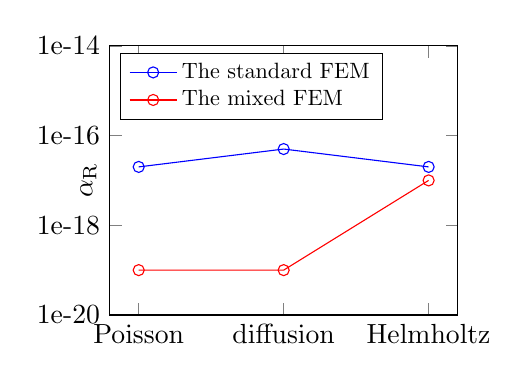
\begin{tikzpicture} 
\begin{axis}
[
    ymode=log,    
    ymin=1e-20,
    ymax=1e-14,
    ytick={1e-20, 1e-18, 1e-16, 1e-14},
    yticklabels={1e-20, 1e-18, 1e-16, 1e-14},      
    legend style={nodes={scale=0.8},at={(0.03,0.85)},anchor=west},
    legend cell align={left},
    height=5cm,
    width=6cm,
    ylabel={$\alpha_{\rm R}$},
    ylabel style={at={(-0.01,0.5)}},    
    xtick={0,1,2,3,4},
    xticklabels={Poisson, diffusion, Helmholtz} 
]
\addplot[blue,mark=o,mark options={color=blue,fill=blue}] coordinates {(0,2.0e-17) (1,5.0e-17) (2,2.0e-17)};
\addplot[red,mark=o,mark options={color=red,fill=red}] coordinates {(0,1.0e-19) (1,1.0e-19) (2,1.0e-17)};
\legend{The standard FEM, The mixed FEM};
\end{axis}
\end{tikzpicture}
}
\vspace{-0.7cm}
\caption{Solution}
\label{alpha_R_benchmark_Poisson}
\end{subfigure}
\hspace{-0.7cm}
\begin{subfigure}[b]{0.35\textwidth}
\scalebox{0.85}{
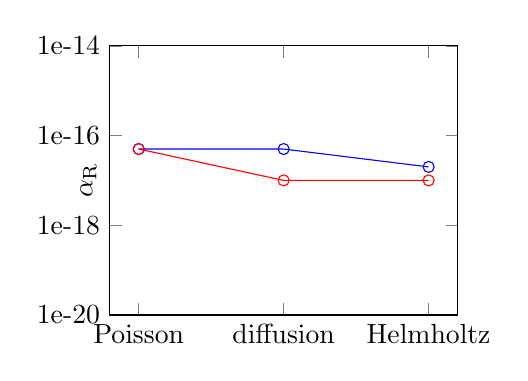
\begin{tikzpicture} 
\begin{axis}
[
    ymode=log,    
    ymin=1e-20,
    ymax=1e-14,
    ytick={1e-20, 1e-18, 1e-16, 1e-14},
    yticklabels={1e-20, 1e-18, 1e-16, 1e-14},      
    legend style={nodes={scale=0.8},at={(0.03,0.85)},anchor=west},
    legend cell align={left},
    height=5cm,
    width=6cm,
    ylabel={$\alpha_{\rm R}$},
    ylabel style={at={(-0.01,0.5)}},    
    xtick={0,1,2,3,4},
    xticklabels={Poisson, diffusion, Helmholtz}
]
\addplot[blue,mark=o,mark options={color=blue,fill=blue}] coordinates {(0,5.0e-17) (1,5.0e-17) (2,2.0e-17)};
\addplot[red,mark=o,mark options={color=red,fill=red}] coordinates {(0,5.0e-17) (1,1.0e-17) (2,1.0e-17)};
\end{axis}
\end{tikzpicture}
}
\vspace{-0.7cm}
\caption{First derivative}
\label{alpha_R_benchmark_diffusion}
\end{subfigure}
\hspace{-0.7cm}
\begin{subfigure}[b]{0.35\textwidth}
\scalebox{0.85}{
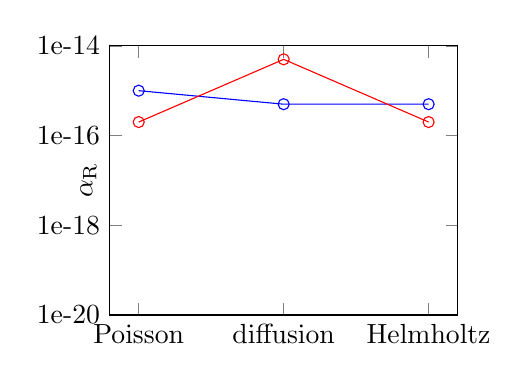
\begin{tikzpicture} 
\begin{axis}
[
    ymode=log,    
    ymin=1e-20,
    ymax=1e-14,
    ytick={1e-20, 1e-18, 1e-16, 1e-14},
    yticklabels={1e-20, 1e-18, 1e-16, 1e-14},      
    legend style={nodes={scale=0.8},at={(0.03,0.85)},anchor=west},
    legend cell align={left},
    height=5cm,
    width=6cm,
    ylabel={$\alpha_{\rm R}$},
    ylabel style={at={(-0.01,0.5)}},    
    xtick={0,1,2,3,4},
    xticklabels={Poisson, diffusion, Helmholtz} 
]
\addplot[blue,mark=o,mark options={color=blue,fill=blue}] coordinates {(0,1.0e-15) (1,5.0e-16) (2,5.0e-16)};
\addplot[red,mark=o,mark options={color=red,fill=red}] coordinates {(0,2.0e-16) (1,5.0e-15) (2,2.0e-16)};
\end{axis}
\end{tikzpicture}
}
\vspace{-0.7cm}
\caption{Second derivative}
\label{alpha_R_benchmark_Helmholtz}
\end{subfigure}
\caption{$\alpha_{\rm R}$ for the benchmark equations.}
\label{alpha_R_benchmark}
\end{figure}

The numerical results in this section show that $\beta_{\rm T}$ can be reached quickly in practice, $\alpha_{\rm R}$ is close to the machine precision and $\beta_{\rm R}$ is relatively fixed. In what follows, $\beta_{\rm R}$ is taken as constant if not stated otherwise.

\subsubsection{Poisson equations of various $u(x)$ and $f(x)$}	    \label{section_scaling}

For the benchmark equations, $\|u_{\rm exc}\|_2$ is of order 1. In this section, we investigate the influence of $\|u_{\rm exc}\|_2$ on the offset $\alpha_{\rm R}$, and also $\|u_{x,\rm exc}\|_2$ when using the mixed FEM.
To cover a wide range of scenarios for both $\|u_{\rm exc}\|_2$ and $\|f\|_2$, we choose 5 cases shown in Table \ref{scaling_cases_Poisson}. Each case contains a coefficient $c_i,~i=1,2, \ldots , 5$, which is varied over several orders of magnitude.
Moreover, Dirichlet boundary conditions are imposed at both ends.
Note that, Case 2 becomes the benchmark Poisson equation when $c_2=1$.

\begin{table}[!ht]
\centering
\caption [w]{Setting of the Poisson equation with different right-hand sides.} 
\label{scaling_cases_Poisson}
 \begin{tabular}{c c c} \hline      
Case & $f(x)$ & $u_{\text{exc}}(x)$ \\ \hline
1 & {$\sin (2 \pi c_1x)$} & ${(2 \pi c_1)}^{-2} \sin (2 \pi c_1x)$\\ \hline
2 & $\makecell{-e^{-{c_2}{(x-1/2)^2}} \cdot \\ \left({4{c_2}^2(x-1/2)^2 -2c_2} \right)}$ & $e^{-{c_2}{{(x-1/2)^2}}}$ \\ \hline
3 & $\sin (2 \pi c_3 x) +1$ & ${(2 \pi c_3)}^{-2}\sin (2 \pi c_3 x)-\frac{x^2}{2}$ \\ \hline
4 & $2 \pi c_4 \sin (2 \pi c_4 x)$ & ${(2 \pi c_4)}^{-1} \sin (2 \pi c_4x)$ \\ \hline
5 & $0$ & ${c_5}^{-1} x$ \\ \hline
\end{tabular}
\end{table}

% \paragraph{The standard FEM}		\label{scaling_std_FEM}
Using the standard FEM, the plots of the offsets $\alpha_{\rm R}$ against $\|u\|_2$ can be found in Fig.~\ref{Fig:py_offset_normal_summary_sm}.
Using the mixed FEM, the plots of the offsets $\alpha_{\rm R}$ against $\|u\|_2$ or $\|u_x\|_2$ can be found in Fig.~\ref{Fig:py_offset_normal_summary_mm}. The relation between $\alpha_{\rm R}$ and $\|u\|_2$ or $\|u_x\|_2$ are summarized in Table~\ref{relation_alpha_R_u_du_l2}.

\begin{figure}[!ht]
    \begin{subfigure}{5.4cm}
        \includegraphics[width=1.0\linewidth]{py_offset_normal_summary_sm_solu.pdf}
        \caption{Solution}
        \label{Fig:py_offset_normal_summary_sm_solu}
    \end{subfigure}
    \hspace{-0.2cm}
    \begin{subfigure}{5.4cm}
        \includegraphics[width=1.0\linewidth]{py_offset_normal_summary_sm_grad.pdf}
        \caption{First derivative}
        \label{Fig:py_offset_normal_summary_sm_grad}
    \end{subfigure}
    \hspace{-0.2cm}
    \begin{subfigure}{5.4cm}
        \includegraphics[width=1.0\linewidth]{py_offset_normal_summary_sm_2ndd.pdf}
        \caption{Second derivative}
        \label{Fig:py_offset_normal_summary_sm_2ndd}
    \end{subfigure}
\caption{Summary of the offsets when using the standard FEM.}
\label{Fig:py_offset_normal_summary_sm}
\end{figure}

\begin{figure}[!ht]
    \begin{subfigure}{5.4cm}
        \includegraphics[width=1.0\linewidth]{py_offset_normal_summary_mm_solu.pdf}
        \caption{Solution}
        \label{Fig:py_offset_normal_summary_mm_solu}
    \end{subfigure}
    \hspace{-0.2cm}
    \begin{subfigure}{5.4cm}
        \includegraphics[width=1.0\linewidth]{py_offset_normal_summary_mm_grad.pdf}
        \caption{First derivative}
        \label{Fig:py_offset_normal_summary_mm_grad}
    \end{subfigure}
    \hspace{-0.2cm}
    \begin{subfigure}{5.4cm}
        \includegraphics[width=1.0\linewidth]{py_offset_normal_summary_mm_2ndd.pdf}
        \caption{Second derivative}
        \label{Fig:py_offset_normal_summary_mm_2ndd}
    \end{subfigure}
\caption{Summary of the offsets when using the mixed FEM.}
\label{Fig:py_offset_normal_summary_mm}
\end{figure}

\newpage

\begin{table}[!ht]
\captionof{table}{Relation between $\alpha_{\rm R}$ and $\|u\|_2$ or $\|u_x\|_2$ for Poisson equations.}
\centering
\begin{tabular}{l c c c}
\hline
 & $u$ & $u_x$ & $u_{xx}$ \\ \hline 
The standard FEM & 2e-17 $\times \|u\|_2$ & 5e-17$\times \|u\|_2$ & 5e-16$\times \|u\|_2$ \\ \hline
The mixed FEM & 1e-18$\times \|u\|_2$ & 1e-16$\times \|u\|_2$ & 5e-16$\times \|u_x\|_2$ \\ \hline
\end{tabular}
\label{relation_alpha_R_u_du_l2}
\end{table}


\subsubsection{Influence of $d(x)$ and $r(x)$}



\section{Sensitivity analysis}       \label{section_sensitivity}

% In this section, we assess the general values for $\alpha_{\rm R}$ and $\beta_{\rm R}$. We start with the preliminary results obtained from three benchmark equations shown in , and then investigate the following factors: order of magnitude, equation type, solution strategy and boundary condition. 

We focus on the benchmark Poisson equation, and the approximation order for each variable is 3.


\subsection{Solution strategy}		\label{section_solver}

The alternative solution method is the iterative Conjugate Gradient (CG) method \cite{ginsburg1963cg}, which is applied when the left-hand side is symmetric and positive definite.
In the standard FEM, it can be applied directly, while in the mixed FEM, since the left-hand side of Eq.~(\ref{matrix equation mix FEM}) is indefinite, it is applied after segregating Eq.~(\ref{matrix equation mix FEM}) based on the Schur complement.
The tolerance of the CG solver is set to be the product of a parameter, denoted by $tol_{prm}$, and the $L_2$ norm of the discrete right-hand side.

\paragraph{The standard FEM}

The comparison of the absolute errors using the two solution approaches are made in Fig.~\ref{py_bench_Pois_SM_error_solution_strategy}, in which $tol_{prm}=$ $10^{-10}$ and $10^{-6}$ are investigated for the CG solver.

\begin{figure}[!ht]
    \begin{subfigure}{5.5cm}
        \includegraphics[width=1.0\linewidth]{py_bench_Pois_SM_error_solution_strategy_solu.pdf}
        \caption{Solution}
        \label{py_bench_Pois_SM_error_solution_strategy_solu}
    \end{subfigure}
    \hspace{-0.2cm}
    \begin{subfigure}{5.5cm}
        \includegraphics[width=1.0\linewidth]{py_bench_Pois_SM_error_solution_strategy_grad.pdf}
        \caption{First derivative}
        \label{py_bench_Pois_SM_error_solution_strategy_grad}
    \end{subfigure}
    \hspace{-0.2cm}
    \begin{subfigure}{5.5cm}
        \includegraphics[width=1.0\linewidth]{py_bench_Pois_SM_error_solution_strategy_2ndd.pdf}
        \caption{Second derivative}
        \label{py_bench_Pois_SM_error_solution_strategy_2ndd}
    \end{subfigure}
\caption{Comparison of the errors using the CG solver and the UMFPACK solver.}
\label{py_bench_Pois_SM_error_solution_strategy}
\end{figure}

When $tol_{prm}$ is adequately small, i.e. $tol_{prm}=10^{-10}$, the CG solver produces basically the same error with the UMFPACK solver except for the second derivative, for which the round-off error increases faster when using the CG solver.
When $tol_{prm}$ is too large, i.e. $tol_{prm}=10^{-6}$, the error contribution due to the iterative solver dominates the discretization error. Furthermore, it is also found that the errors of higher-order elements are more easier to be affected by larger $tol_{prm}$.

\paragraph{The mixed FEM}

The resulting system of equations after segregating Eq.~(\ref{matrix equation mix FEM}) reads
\begin{subequations}
 \begin{align}
  B^{\top} M^{-1} B U &= B^{\top} M^{-1} G - H, 	\label{schur_complement_solution} \\
  MV&=G-BU,						\label{schur_complement_gradient}
\end{align}						\label{schur_complement_solu_grad}%
\end{subequations}
for which Eq. (\ref{schur_complement_solution}) is solved in the first place to obtain $U$, which is then substituted into Eq. (\ref{schur_complement_gradient}) to obtain $V$.


We first investigate the influence of $tol_{prm}$ of the CG solver on the solution accuracy when the left-hand side is $B^{\top}M^{-1}B$ (Schur complement). In this case, the UMFPACK solver is used to solve the system of equations for the left-hand side being $M$.  
For $tol_{prm}$ being $10^{-16}$ and $10^{-10}$, the errors are shown in Fig. \ref{Fig:py_bench_Pois_MM_error_solution_strategy_schur_variant_other_UMF}, in comparison with that obtained from solving the monolithic Eq. (\ref{matrix equation mix FEM}) directly.
It shows that the monolithic solution approach yields by far the most accurate solution and derivative values.
Remarkably, the round-off error for $v_{x}$ increases fastest using the Schur complement approach even though $tol_{prm}$ is sufficiently small, i.e. $tol_{prm}=10^{-16}$.
When $tol_{prm}$ is less strict, i.e. $tol_{prm}=10^{-10}$, the iteration error dominates the discretization error before the round-off error.

\begin{figure}[!ht]
    \begin{subfigure}{5.5cm}
        \includegraphics[width=1.0\linewidth]{py_bench_Pois_MM_error_solution_strategy_schur_variant_other_UMF_solu.pdf}
        \caption{Solution}
        \label{Fig:py_bench_Pois_MM_error_solution_strategy_schur_variant_other_UMF_solu}
    \end{subfigure}
    \hspace{-0.2cm}
    \begin{subfigure}{5.5cm}
        \includegraphics[width=1.0\linewidth]{py_bench_Pois_MM_error_solution_strategy_schur_variant_other_UMF_grad.pdf}
        \caption{First derivative}
        \label{Fig:py_bench_Pois_MM_error_solution_strategy_schur_variant_other_UMF_grad}
    \end{subfigure}
    \hspace{-0.2cm}
    \begin{subfigure}{5.5cm}
        \includegraphics[width=1.0\linewidth]{py_bench_Pois_MM_error_solution_strategy_schur_variant_other_UMF_2ndd.pdf}
        \caption{Second derivative}
        \label{Fig:py_bench_Pois_MM_error_solution_strategy_schur_variant_other_UMF_2ndd}
    \end{subfigure}
\caption{Influence of the CG solver on the solution accuracy using the mixed FEM when the left-hand side is the Schur complement.}
\label{Fig:py_bench_Pois_MM_error_solution_strategy_schur_variant_other_UMF}
\end{figure}

% \newpage
Next, we investigate the influence of $tol_{prm}$ of the CG solver when the left-hand side is $M$. In this case, the CG solver with $tol_{prm}$ being $10^{-16}$ is used to solve the system of equations with the left-hand side being $B^{\top}M^{-1}B$. For the same tolerances, the errors are basically the same with that shown in Fig.~\ref{Fig:py_bench_Pois_MM_error_solution_strategy_schur_variant_other_UMF}.

In summary, when $tol_{prm}$ is strict enough, for the standard FEM, the CG solver gives the same accuracy for $u$ and $u_{x}$ as the UMFPACK solver , while the UMFPACK solver produces higher accuracy for $u_{xx}$; for the mixed FEM, the accuracy for all the three variables is the highest when using the monolithic approach. When $tol_{prm}$ is less strict, the applications of the CG solver on both the standard and mixed FEM methods introduce iteration errors.

\subsection{Boundary conditions}	\label{section_BC}

In this section, two aspects of the influence of the boundary conditions on the round-off error are investigated: first the method of implementing the Dirichlet boundary conditions, and secondly types of boundary conditions. 

For the first aspect, using Weak form 2 for $\rho=50$ and $10^6$, the discretization errors are depicted in Fig.~\ref{py_bench_Pois_SM_error_boundary_weak}, in comparison with that using Weak form 1. As can be seen, both weak and strong imposition of the Dirichlet boundary condition yield the same trend line for the round-off error for the solution and its derivatives, and the magnitude of the penalty parameter in the weak imposition makes no difference. In addition, small penalty parameters might lead to larger truncation errors for $u$, but the difference diminishes when the penalty parameter is large enough.

\begin{figure}[!ht]
    \begin{subfigure}{5.5cm}
        \includegraphics[width=1.0\linewidth]{py_bench_Pois_SM_error_boundary_weak_solu.pdf}
        \caption{Solution}
        \label{py_bench_Pois_SM_error_boundary_weak_solu}
    \end{subfigure}
    \hspace{-0.2cm}
    \begin{subfigure}{5.5cm}
        \includegraphics[width=1.0\linewidth]{py_bench_Pois_SM_error_boundary_weak_grad.pdf}
        \caption{First derivative}
        \label{py_bench_Pois_SM_error_boundary_weak_grad}
    \end{subfigure}
    \hspace{-0.2cm}
    \begin{subfigure}{5.5cm}
        \includegraphics[width=1.0\linewidth]{py_bench_Pois_SM_error_boundary_weak_2ndd.pdf}
        \caption{Second derivative}
        \label{py_bench_Pois_SM_error_boundary_weak_2ndd}
    \end{subfigure}
\caption{Comparison of the errors for imposing the Dirichlet boundary condition strongly and weakly.}
\label{py_bench_Pois_SM_error_boundary_weak}
\end{figure}

To construct the problem for the second aspect, the Dirichlet boundary condition at the left boundary ($x=0$) is kept while the Dirichlet boundary condition at the right boundary ($x=1$) has been replaced by the Neumann boundary condition $u_x (1) = -e^{-1/4}$, leading to the same solution and derivative profiles. 


% \newpage
\paragraph{The standard FEM}
Using the standard FEM, the offsets $\alpha_{\rm R}$ for the two types of boundary conditions are depicted in Fig.~\ref{boundary_type_benchmark_Poisson_std}. 
For the Dirichlet/Neumann boundary condition, the offsets $\alpha_{\rm R}$ for $u$ and $u_x$ are slightly larger than that for the Dirichlet/Dirichlet boundary condition by a factor of 3.5 and 2, respectively. The offsets $\alpha_{\rm R}$ for $u_{xx}$ are identical for the two types of boundary conditions.

\paragraph{The mixed FEM}
Using the mixed FEM, the offsets $\alpha_{\rm R}$ for the two types of boundary conditions are depicted in Fig.~\ref{boundary_type_benchmark_Poisson_mix}.
As can be seen, the type of boundary conditions plays a more important role for $\alpha_{\rm R}$ for the solution than $\alpha_{\rm R}$ for other variables.


\begin{figure}[!ht]
\hspace{2.2cm}
% \centering
\begin{subfigure}[b]{0.4\textwidth}
\scalebox{0.9}{
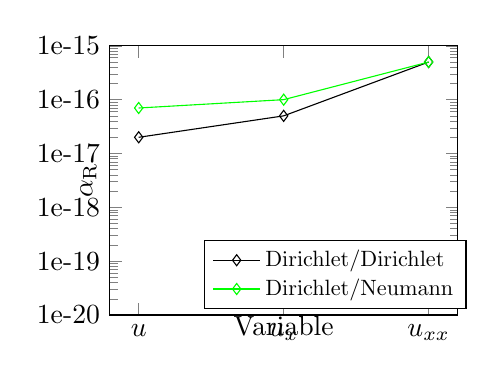
\begin{tikzpicture} 
\begin{axis}
[
    ymode=log,    
    ymin=1e-20,
    ymax=1e-15,
    ytick={1e-20,1e-19,1e-18,1e-17,1e-16,1e-15},
    yticklabels={1e-20,1e-19,1e-18,1e-17,1e-16,1e-15},      
    legend style={nodes={scale=0.8},at={(0.27,0.15)},anchor=west},
    legend cell align={left},
    height=5cm,
    width=6cm,
    ylabel={$\alpha_{\rm R}$},
    ylabel style={at={(-0.01,0.5)}},    
    xtick={0,1,2,3,4},
    xticklabels={$u$,$u_x$, $u_{xx}$, $4$, ${5}$},
    xlabel={Variable},
    xlabel style={at={(0.5,0.03)}},    
]
\addplot[black,mark=diamond,mark options={color=black,fill=black}] coordinates {(0,2.0e-17) (1,5.0e-17) (2,5.0e-16)};
\addplot[green,mark=diamond,mark options={color=green,fill=green}] coordinates {(0,7.0e-17) (1,1.0e-16) (2,5.0e-16)};
\legend{Dirichlet/Dirichlet, Dirichlet/Neumann};
\end{axis}
\end{tikzpicture}
}
\caption{The standard FEM}
\label{boundary_type_benchmark_Poisson_std}
\end{subfigure}
\hspace{-1.0cm}
\begin{subfigure}[b]{0.4\textwidth}
\scalebox{0.9}{
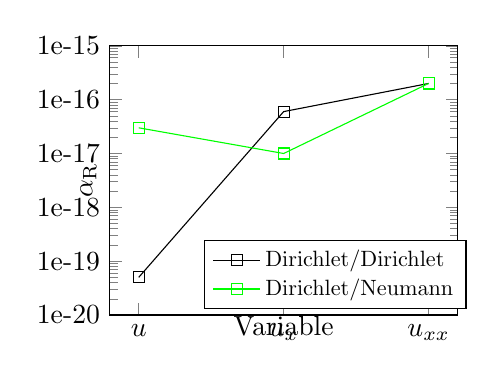
\begin{tikzpicture} 
\begin{axis}
[
    ymode=log,    
    ymin=1e-20,
    ymax=1e-15,
    ytick={1e-20,1e-19,1e-18,1e-17,1e-16,1e-15},
    yticklabels={1e-20,1e-19,1e-18,1e-17,1e-16,1e-15},        
    legend style={nodes={scale=0.8},at={(0.27,0.15)},anchor=west},
    legend cell align={left},
    height=5cm,
    width=6cm,
    ylabel={$\alpha_{\rm R}$},
    ylabel style={at={(-0.01,0.5)}},    
    xtick={0,1,2,3,4},
    xticklabels={$u$,$u_x$, $u_{xx}$, $4$, ${5}$},
    xlabel={Variable},
    xlabel style={at={(0.5,0.03)}},    
]
\addplot[black,mark=square,mark options={color=black,fill=black}] coordinates {(0, 5.0e-20) (1, 6.0e-17) (2, 2.0e-16)};
\addplot[green,mark=square,mark options={color=green,fill=green}] coordinates {(0, 3.0e-17) (1, 1.0e-17) (2, 2.0e-16)};
\legend{Dirichlet/Dirichlet, Dirichlet/Neumann};
\end{axis}
\end{tikzpicture}
}
\caption{The mixed FEM}
\label{boundary_type_benchmark_Poisson_mix}
\end{subfigure}
\caption{Comparison of the errors for imposing Dirichlet/Dirichlet and Dirichlet/Neumann boundary conditions.}
\label{boundary_type_benchmark_Poisson}
\end{figure}


In summary, $\alpha_{\rm R}$ are relatively independent of the variations in the type of boundary conditions and the method Dirichlet boundary conditions are implemented, which is an important prerequisite for our a posteriori refinement strategy to be applicable for a wide range of problems.

To conclude the sections on sensitivity analysis, the factors that cannot be mitigated are the tolerances for the iterative linear solver, that can be mitigated are the order of magnitude, and that are relatively irrelevant are the boundary conditions.

% \newpage
\section{Approach to find the optimal number of DoFs}                 \label{approach_finding_optimal_number_of_DoFs}

\subsection{Strategy}           \label{section_strategy}

Moreover, $\alpha_{\rm T}$ can be inverted at the beginning of the second phase by using
\begin{equation}
 \alpha_{\rm T} = {E_{\rm c}}/{N_{\rm c}}^{- \beta_{\rm T}},		\label{formula_offset_truncation_error}
\end{equation}
where ${E_{\rm c}}$ and ${N_{\rm c}}$ are the corresponding $E_h$ and $N_h$.


Obviously, $N_{\rm opt}$ happens when the sum of the truncation error and the round-off error ($E_{\rm T}+E_{\rm R}$) is the smallest. By solving
\begin{equation}
    \frac{d(E_{\rm T}+E_{\rm R})}{dN}=0,    \label{derivative_condition_N_opt}
\end{equation}
we can predict
\begin{subequations}
\begin{align}
 N_{\rm opt} = \left( \frac{\alpha_{\rm T} \beta_{\rm T}}{\alpha _{\rm R} \beta_{\rm R}} \right)^{\frac{1}{\beta_{\rm T} + \beta_{\rm R}}},
\end{align}
and hence, the highest attainable accuracy
\begin{align}
 E_{\rm min} = \alpha_{\rm T} {N_{\rm opt}}^{- {\beta _{\rm T}}}+\alpha_{\rm R} {N_{\rm opt}}^{{\beta _{\rm R}}}.
\end{align}
\end{subequations}


\subsection{A posteriori algorithm for finding the optimal number of degrees of freedom}		\label{section_algorithm}

Based on the validation experiments from the previous section, we introduce a novel a posteriori algorithm for determining $E_{\rm min}$ for the solution and its first and second derivative without performing the brute-force mesh refinement. 
Table \ref{settings_algorithm} gives the default settings and the required custom input of the algorithm.

\begin{table}[!ht]
\captionof{table}{Settings of the algorithm.}
\label{settings_algorithm}
  \centering
  \begin{tabular}{lL{5cm}L{6cm}}
    \toprule
    Item & Default & Custom  \\
    \midrule
    Problem & - & \tabitem the differential equation to be solved \\
     &  & \tabitem its associated boundary conditions \\\hline
    Grid & \tabitem initial number of vertices: 2 & - \\
     & \tabitem the vertices are equidistant &  \\\hline
    FEM & \tabitem the maximum $N_h$, denoted by $N_{\rm max}$, : $10^8$ & \tabitem standard or mixed formulation \\
    & \tabitem Dirichlet boundary conditions are imposed strongly & \tabitem an ordered array of element degrees $\{p_{\min}, \ldots, p_{\rm max}\}$ \\\hline
    Computer precision & IEEE-754 double precision & - \\\hline
    Solver & UMFPACK & - \\\hline
    $var$ & - & \tabitem chosen from $\{u,~u_x,~u_{xx}\}$ \\     
    & & \tabitem error tolerance $tol_{var}$ \\     
    \bottomrule
  \end{tabular}
\end{table}

% \newpage
Furthermore, we use the following coefficients in the algorithm:		% the following input
\begin{itemize}
  \renewcommand\labelitemi{--}
  \item a minimal number of $h$-refinements before `\textit{NORMALIZATION}' and carrying out `\textit{PREDICTION}', denoted by $REF_{\rm min}$, with the following default values:
  \begin{equation}
  \begin{aligned}
      REF_{\rm min} &=
      \begin{cases*}
	9-p & for p $<$ 6, \\
	4 & otherwise.
      \end{cases*}
  \end{aligned}
  \end{equation} 
  We choose this parameter mainly because the error might increase, or decrease faster than the theoretical order of convergence for coarse refinements, especially for lower-order elements.
%   \item a stopping criterion $c_s$ for seeking the scaling factor $\|var_{\rm exc}\|_{2}$ in Table~\ref{scaling schemes std and mix FEM}, its value is 0.001 by default. We choose this parameter because the analytical solution does not exist for most practical problems.
  \item a relaxation coefficient $c_r$ for seeking the theoretical order of convergence, with the following default values: 
    \begin{equation}
    \begin{aligned}
	c_r &=
	\begin{cases*}
	  0.9 & for p $<$ 4, \\
	  0.7 & for 4 $\leqslant$ p $<$ 10, \\
	  0.5 & otherwise.
	\end{cases*}
    \end{aligned}
    \end{equation}
  \item the offset $\alpha _{\rm R}$, see Table \ref{relation_alpha_R_u_du_l2} for the default values.
\end{itemize}

% \newpage
The procedure of our algorithm consists of four steps, which are explained below:

\paragraph{Step-1} `\textit{INPUT}'. In this step, the custom input has to be provided.
\paragraph{Step-2} `\textit{NORMALIZATION}'. The function of this step is to find the scaling factor to normalize problems of different orders of magnitude for the variable. The specific procedure can be found in Algorithm \ref{algo_scaling_factor}, where elements of degree $p_{\rm min}$ are used. 

\vspace{0.2cm}
\begin{algorithm}[H]
\caption{NORMALIZATION}
\label{algo_scaling_factor}
\While{$N_h<N_{\rm max}$}
{
    \eIf{$\left|\frac{\|var_{h}\|_{2} - \|var_{2h}\|_{2}}{\|var_{h}\|_{2}} \right| < c_s$}
    {
        $\|var_{\rm exc}\|_{2}$ $\gets$ $\|var_{h}\|_{2}$\;
        break\;
    }
    {
        $h$ $\gets$ $h/2$\;
        calculate $\|var_h\|_{2}$ using Eq. (\ref{formula_abs_error_analytical}) without scaling\;    
    }
}
\end{algorithm}
                                                                   
\paragraph{Step-3} `\textit{PREDICTION}'. This step finds $E_{\rm min}$ for each $var$ and $p$ of interest, as illustrated in Fig.~\ref{sketch_discretization_error_one_p}.
The procedure for carrying out this step can be found in Algorithm \ref{block_PREDICTION}.

\vspace{0.2cm}
\begin{algorithm}[H]
\caption{PREDICTION}			% Seeking the analytical order of convergence Predicting $N_{\rm opt}$ and $E_{\rm min}$
\label{block_PREDICTION}
    \While{$\widetilde {E_{h}}>E_{\rm R}$ \textbf{\textup{and}} $N_h<N_{\rm max}$}
    {
        $\widetilde{Q}$ $\gets$ $\log _2 \left( {\widetilde {E_{2h}}}/{\widetilde {E_{h}}} \right)$\;
        \eIf
        {
            $\widetilde{Q} \geqslant \beta_{\rm T} \times c_r$
        }
        {
            $N_{\rm c} \gets N_h$\;
            $E_{\rm c} \gets \widetilde {E_{h}}$\;
            $\alpha_{\rm T}$ $\gets$ ${E_{\rm c}}/{N_{\rm c}}^{- \beta_{\rm T}}$\;
            $N_{\rm opt} \gets \left( \frac{\alpha_{\rm T} \beta_{\rm T}}{\alpha _{\rm R} \beta_{\rm R}} \right)^{\frac{1}{\beta_{\rm R} + \beta_{\rm T}}}$\;
            $E_{\rm min} \gets \alpha_{\rm T} {N_{\rm opt}}^{- {\beta _{\rm T}}} + \alpha_{\rm R} {N_{\rm opt}}^{{\beta _{\rm R}}}$\;

        }
        {
            $h$ $\gets$ $h/2$\;
            calculate $\widetilde {E_{h}}$ using Eq.~(\ref{formula_abs_error_numerical}) with proper scaling schemes\;
        }
	}    
\end{algorithm}

\paragraph{Step-4} `\textit{OUTPUT}'. In this step, we output $E_{\rm min}$ obtained from $Step$-3.

\section{Validation}		\label{section_validation}

In what follows, we validate the strategy discussed in Section \ref{section_behaviour_discretization_error} by using the following Helmholtz problem:
\begin{equation}
  \left((0.01+x)(1.01-x) u_x \right)_x -(0.01i) u(x) = 1.0,\qquad x \in I = (0,1),	\label{1D_Helmholtz_equation_application}
\end{equation}
with homogeneous Dirichlet and Neumann boundary conditions imposed as follows: $u(0)=0$ and $u_x(1)=0$.

Both the standard FEM and the mixed FEM are investigated, and the element degree $p$ has a range of $\{1, 2, \ldots, 5\}$. Variables $u$, $u_x$ and $u_{xx}$ are all investigated, for which $tol_{var}$ is set to be $10^{-9}$. 

Using the prediction approach and the brute-force approach, $E_{\rm min}$ are compared in Fig.~\ref{E_min_application}. As can be seen, $E_{\rm min}$ can be predicted correctly.

\begin{figure}[!ht]
\hspace{0.0cm}
\begin{subfigure}[b]{0.35\textwidth}
\scalebox{0.9}{
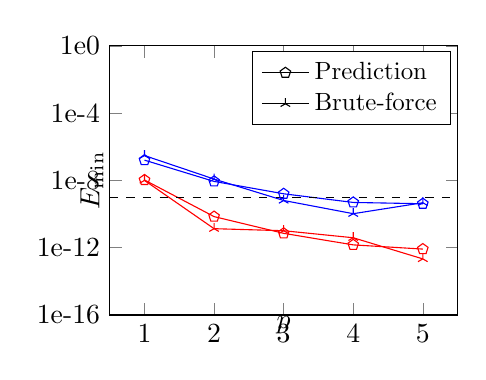
\begin{tikzpicture} 
\begin{axis}
[
    xmin=-0.5,
    xmax=4.5,
    ymode=log,
    ymin=1e-16,
    ymax=1,
    ytick={1e-16, 1e-12, 1e-8, 1e-4, 1e0},
    yticklabels={1e-16, 1e-12, 1e-8, 1e-4, 1e0},    
    legend style={nodes={scale=0.9}},
    legend cell align={left},    
    height=5cm,
    width=6cm,
    ylabel={$E_{\min}$}, 
    ylabel style={at={(0.01,0.5)}},  
    xtick={0,1,2,3,4},
    xticklabels={$1$, $2$, $3$, $4$, ${5}$},
    xlabel={$p$},
    xlabel style={at={(0.5,0.03)}}, 
]
\addplot[black,mark=pentagon,mark options={color=black,fill=black}] coordinates {(0,2.1e-25)};
\addplot[black,mark=Mercedes star,mark options={color=black,fill=black}] coordinates {(0,2.1e-25)};

\addplot[blue,mark=pentagon,mark options={color=blue,fill=blue}] coordinates {(0,1.6e-7) (1,8.7e-9) (2,1.6e-9) (3,4.9e-10) (4,4.1e-10)}; 
\addplot[blue,mark=Mercedes star,mark options={color=blue,fill=blue}] coordinates {(0,3e-7) (1,1.2e-8) (2,6.4e-10) (3,1.05e-10) (4,4.7e-10)}; 

\addplot[red,mark=pentagon,mark options={color=red,fill=red}] coordinates {(0,1.06e-8) (1,7.05e-11) (2,7.13e-12) (3,1.47e-12) (4,8.27e-13)}; 
\addplot[red,mark=Mercedes star,mark options={color=red,fill=red}] coordinates {(0,1.0e-8) (1,1.35e-11) (2,1.02e-11) (3,3.9e-12) (4,2.16e-13)}; 
\addplot[color=black, dashed] coordinates {(-0.5, 1e-9) (4.5, 1e-9)};
\legend{Prediction,Brute-force};
\end{axis}
\end{tikzpicture}
}
\vspace{-0.2cm}
\caption{Solution}
\end{subfigure}
\hspace{-0.7cm}
\begin{subfigure}[b]{0.35\textwidth}
\scalebox{0.9}{
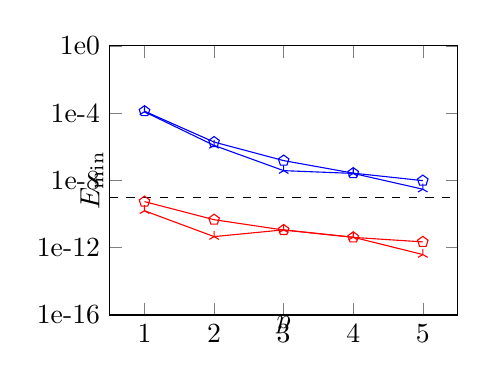
\begin{tikzpicture} 
\begin{axis}
[
    xmin=-0.5,
    xmax=4.5,
    ymode=log,
    ymin=1e-16,
    ymax=1,
    ytick={1e-16, 1e-12, 1e-8, 1e-4, 1e0},
    yticklabels={1e-16, 1e-12, 1e-8, 1e-4, 1e0},
    legend style={nodes={scale=0.8}},
    legend cell align={left},    
    height=5cm,
    width=6cm,
    ylabel={$E_{\min}$},
    ylabel style={at={(0.01,0.5)}},  
    xtick={0,1,2,3,4},
    xticklabels={$1$, $2$, $3$, $4$, ${5}$},
    xlabel={$p$},
    xlabel style={at={(0.5,0.03)}},    
]
\addplot[blue,mark=pentagon,mark options={color=blue,fill=blue}] coordinates {(0,1.3e-4) (1,1.9e-6) (2,1.5e-7) (3,2.7e-8) (4,9.7e-9)}; 
\addplot[blue,mark=Mercedes star,mark options={color=blue,fill=blue}] coordinates {(0,1.2e-4) (1,1.2e-6) (2,3.8e-8) (3,2.6e-8) (4,3.0e-9)}; 

\addplot[red,mark=pentagon,mark options={color=red,fill=red}] coordinates {(0,5.47e-10) (1,4.62e-11) (2,1.12e-11) (3,4.11e-12) (4,2.21e-12)}; 
\addplot[red,mark=Mercedes star,mark options={color=red,fill=red}] coordinates {(0,1.57e-10) (1,4.56e-12) (2,1.15e-11) (3,4.2e-12) (4,3.91e-13)}; 
\addplot[color=black, dashed] coordinates {(-0.5, 1e-9) (4.5, 1e-9)};
\end{axis}
\end{tikzpicture}
}
\vspace{-0.2cm}
\caption{First derivative}
\end{subfigure}
\hspace{-0.7cm}
\begin{subfigure}[b]{0.35\textwidth}
\scalebox{0.9}{
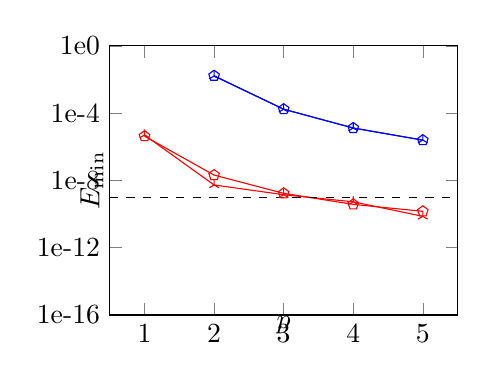
\begin{tikzpicture} 
\begin{axis}
[
    xmin=-0.5,
    xmax=4.5,
    ymode=log,
    ymin=1e-16,
    ymax=1,
    ytick={1e-16, 1e-12, 1e-8, 1e-4, 1e0},
    yticklabels={1e-16, 1e-12, 1e-8, 1e-4, 1e0},
    legend style={nodes={scale=0.8}},
    legend cell align={left},    
    height=5cm,
    width=6cm,
    ylabel={$E_{\min}$},
    ylabel style={at={(0.01,0.5)}},  
    xtick={0,1,2,3,4},
    xticklabels={$1$, $2$, $3$, $4$, ${5}$},
    xlabel={$p$},
    xlabel style={at={(0.5,0.03)}}, 
]
\addplot[blue,mark=pentagon,mark options={color=blue,fill=blue}] coordinates {(0) (1,1.66e-2) (2,1.71e-4) (3,1.3e-5) (4,2.46e-6)}; 
\addplot[blue,mark=Mercedes star,mark options={color=blue,fill=blue}] coordinates {(1,1.6e-2) (2,1.7e-4) (3,1.3e-5) (4,2.5e-6)}; 

\addplot[red,mark=pentagon,mark options={color=red,fill=red}] coordinates {(0,4.25e-6) (1,2.07e-8) (2,1.70e-9) (3,3.75e-10) (4,1.45e-10)}; 
\addplot[red,mark=Mercedes star,mark options={color=red,fill=red}] coordinates {(0,5e-6) (1,5.36e-9) (2,1.41e-9) (3,5.33e-10) (4,7.29e-11)}; 
\addplot[color=black, dashed] coordinates {(-0.5, 1e-9) (4.5, 1e-9)};
\end{axis}
\end{tikzpicture}
}
\vspace{-0.2cm}
\caption{Second derivative}
\end{subfigure}
\caption{Comparison of $E_{\rm min}$ for Eq. (\ref{1D_Helmholtz_equation_application}) using the algorithm and the brute-force refinement. The blue color denotes the standard FEM, and the red color denotes the mixed FEM.}
\label{E_min_application}
\end{figure}

% \newpage

The CPU time required by the prediction approach (PRED) and the brute-force approach (BF) is shown in Fig.~\ref{CPU_algorithm_brute_force}. Next to time PRED, and the computation time for the optimal grid (PRED+) using the prediction approach is also given.
As can be seen, both time BF and time PRED+ decrease with increasing element degree. Time PRED+ is much smaller compared to time BF, see Fig.~\ref{Percentage_CPU_Saved} for the percentage of the CPU time saved by PRED+, which shows a saving of the CPU time basically more than 60\% and 40\% for the standard FEM and the mixed FEM, respectively. Last but not least, time PRED is negligible compared to time PRED+.

\begin{figure}[!ht]
\hspace{0.0cm}
\begin{subfigure}[b]{0.35\textwidth}
\scalebox{0.9}{
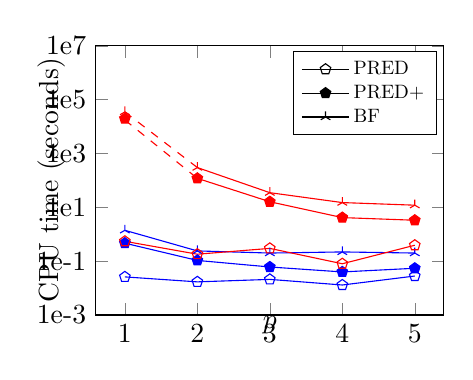
\begin{tikzpicture} 
\begin{axis}
[
    ymode=log,
    ymin=1e-3,
    ymax=1e7,
    ytick={1e-3, 1e-1, 1e1, 1e3, 1e5, 1e7},
    yticklabels={1e-3, 1e-1, 1e1, 1e3, 1e5, 1e7},
    legend style={nodes={scale=0.7}},
    legend cell align={left},
    height=5cm,
    width=6cm,
    ylabel={CPU time (seconds)},
    ylabel style={below},    
    xtick={0,1,2,3,4},
    xticklabels={$1$, $2$, $3$, $4$, ${5}$},
    xlabel={$p$},
    xlabel style={at={(0.5,0.03)}},   
]
\addplot[black,mark=pentagon,mark options={color=black,fill=black}] coordinates {(0,2.1e-25)}; 
\addplot[black,mark=pentagon*,mark options={color=black,fill=black}] coordinates {(0,2.1e-25)};
\addplot[black,mark=Mercedes star,mark options={color=black,fill=black}] coordinates {(0,2.1e-25)}; 

\addplot[blue,mark=pentagon,mark options={color=blue,fill=blue}] coordinates {(0,0.026) (1,0.017) (2,0.021) (3,0.013) (4,0.028)}; 
\addplot[blue,mark=pentagon*,mark options={color=blue,fill=blue}] coordinates {(0,0.026+0.439343) (1,0.017+0.08932) (2,0.021+0.0397) (3,0.013+0.026735) (4,0.028+0.02639)};
\addplot[blue,mark=Mercedes star,mark options={color=blue,fill=blue}] coordinates {(0,1.4) (1,0.24) (2,0.2) (3,0.22) (4,0.2)}; 

\addplot[red,mark=pentagon,mark options={color=red,fill=red}] coordinates {(0,0.546) (1,0.181) (2,0.298) (3,0.08) (4,0.39)}; 
\addplot[red,mark=pentagon*,mark options={color=red,fill=red}] coordinates {(0,0.546+19600)};
\addplot[red,mark=pentagon*,mark options={color=red,fill=red}] coordinates {(1,0.181+119) (2,0.298+15.8) (3,0.08+4.07) (4,0.39+2.92)};
\draw [red,dashed] (axis cs:0,0.546+17600) -- (axis cs:1,0.181+119);
\addplot[red,mark=Mercedes star,mark options={color=red,fill=red}] coordinates {(0,35000)};
\addplot[red,mark=Mercedes star,mark options={color=red,fill=red}] coordinates {(1,300) (2,35) (3,15) (4,12)};
\draw [red,dashed] (axis cs:0,35000) -- (axis cs:1,300);

\legend{PRED, PRED+, BF};
\end{axis}
\end{tikzpicture}
}
\vspace{-0.2cm}
\caption{Solution}
\end{subfigure}
\hspace{-0.7cm}
\begin{subfigure}[b]{0.35\textwidth}
\scalebox{0.9}{
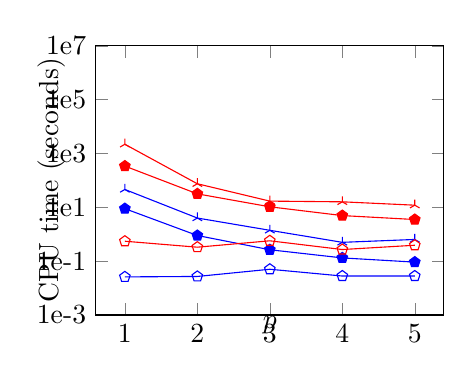
\begin{tikzpicture} 
\begin{axis}
[
    ymode=log,
    ymin=1e-3,
    ymax=1e7,
    ytick={1e-3, 1e-1, 1e1, 1e3, 1e5, 1e7},
    yticklabels={1e-3, 1e-1, 1e1, 1e3, 1e5, 1e7},
    legend style={nodes={scale=0.7}},
    legend cell align={left},
    height=5cm,
    width=6cm,
    ylabel={CPU time (seconds)},
    ylabel style={below},    
    xtick={0,1,2,3,4},
    xticklabels={$1$, $2$, $3$, $4$, ${5}$},
    xlabel={$p$},
    xlabel style={at={(0.5,0.03)}},   
]
\addplot[blue,mark=pentagon,mark options={color=blue,fill=blue}] coordinates {(0,0.026) (1,0.027) (2,0.050) (3,0.028) (4,0.028)}; 
\addplot[blue,mark=pentagon*,mark options={color=blue,fill=blue}] coordinates {(0,0.026+8.9) (1,0.027+0.87) (2,0.05+0.215) (3,0.028+0.104) (4,0.028+0.064)};
\addplot[blue,mark=Mercedes star,mark options={color=blue,fill=blue}] coordinates {(0,46) (1,4) (2,1.4) (3,0.5) (4,0.64)}; 

\addplot[red,mark=pentagon,mark options={color=red,fill=red}] coordinates {(0,0.55) (1,0.33) (2,0.57) (3,0.27) (4,0.39)}; 
\addplot[red,mark=pentagon*,mark options={color=red,fill=red}] coordinates {(0,0.55+340) (1,0.33+31.3) (2,0.57+9.88) (3,0.27+4.66) (4,0.39+3.13)};
\addplot[red,mark=Mercedes star,mark options={color=red,fill=red}] coordinates {(0,2200) (1,75) (2,17) (3,16) (4,12)}; 
\end{axis}
\end{tikzpicture}
}
\vspace{-0.2cm}
\caption{First derivative}
\end{subfigure}
\hspace{-0.7cm}
\begin{subfigure}[b]{0.35\textwidth}
\scalebox{0.9}{
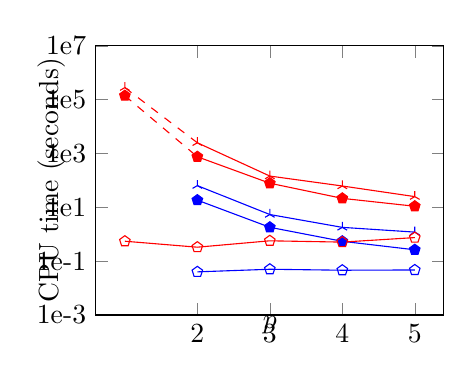
\begin{tikzpicture} 
\begin{axis}
[
    ymode=log,
    ymin=1e-3,
    ymax=1e7,
    ytick={1e-3, 1e-1, 1e1, 1e3, 1e5, 1e7},
    yticklabels={1e-3, 1e-1, 1e1, 1e3, 1e5, 1e7},
    legend style={nodes={scale=0.7}},
    legend cell align={left},
    height=5cm,
    width=6cm,
    ylabel={CPU time (seconds)},
    ylabel style={below},     
    xtick={1,2,3,4},
    xticklabels={$2$, $3$, $4$, ${5}$},
    xlabel={$p$},
    xlabel style={at={(0.5,0.03)}},     
]
\addplot[blue,mark=pentagon,mark options={color=blue,fill=blue}] coordinates {(1,0.04) (2,0.05) (3,0.046) (4,0.047)}; 
\addplot[blue,mark=pentagon*,mark options={color=blue,fill=blue}] coordinates {(1,0.04+18.4184) (2,0.05+1.76016) (3,0.046+0.500414) (4,0.047+0.217396)}; 
\addplot[blue,mark=Mercedes star,mark options={color=blue,fill=blue}] coordinates {(1,64) (2,5.4) (3,1.8) (4,1.2)}; 

\addplot[red,mark=pentagon,mark options={color=red,fill=red}] coordinates {(0,0.55) (1,0.33) (2,0.57) (3,0.51) (4,0.75)}; 
\addplot[red,mark=pentagon*,mark options={color=red,fill=red}] coordinates {(0,0.55+140000)};
\addplot[red,mark=pentagon*,mark options={color=red,fill=red}] coordinates {(1,0.33+755) (2,0.57+78) (3,0.51+21) (4,0.75+10.2)};
\draw [red,dashed] (axis cs:0,0.55+140000) -- (axis cs:1,0.33+755);
\addplot[red,mark=Mercedes star,mark options={color=red,fill=red}] coordinates {(0,280000)};
\addplot[red,mark=Mercedes star,mark options={color=red,fill=red}] coordinates {(1,2500) (2,145) (3,62) (4,25)};
\draw [red,dashed] (axis cs:0,280000) -- (axis cs:1,2500);
\end{axis}
\end{tikzpicture}
}
\vspace{-0.2cm}
\caption{Second derivative}
\end{subfigure}
\caption{Comparison of the CPU time to obtain $E_{\rm min}$ for Eq. (\ref{1D_Helmholtz_equation_application}) using the algorithm and the brute-force refinement. The blue color denotes the standard FEM, and the red color denotes the mixed FEM.}
\label{CPU_algorithm_brute_force}
\end{figure}


\vspace{-0.5cm}
\begin{figure}[!ht]
\centering
\scalebox{0.9}{
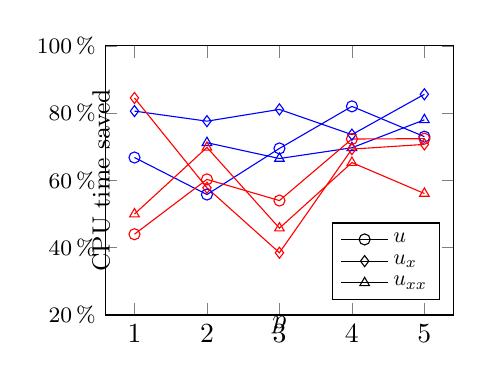
\begin{tikzpicture}
\begin{axis}
[
    ymin=20,
    ymax=100,
    legend style={nodes={scale=0.8},at={(0.65,0.2)},anchor=west},
    legend cell align={left},
    height=5cm,
    width=6cm,
    ylabel={CPU time saved},
    ylabel style={at={(0.04,0.5)},font=\small},
    y tick label style={font=\footnotesize},
    yticklabel=\pgfmathprintnumber{\tick}\,$\%$,
    xtick={0,1,2,3,4},
    xticklabels={$1$, $2$, $3$, $4$, ${5}$},
    xlabel={$p$},
    xlabel style={at={(0.5,0.03)}}, 
]
\addplot[black,mark=o,mark options={color=black,fill=black}] coordinates {(0,2.1e-25)};
\addplot[black,mark=diamond,mark options={color=black,fill=black}] coordinates {(0,2.1e-25)};
\addplot[black,mark=triangle,mark options={color=black,fill=black}] coordinates {(0,2.1e-25)};


\addplot[blue,mark=o,mark options={color=blue,fill=blue}] coordinates {(0,66.8) (1,55.8) (2,69.5) (3,82.0) (4,73.0)};
\addplot[blue,mark=diamond,mark options={color=blue,fill=blue}] coordinates {(0,80.6) (1,77.6) (2,81.1) (3,73.6) (4,85.6)};
\addplot[blue,mark=triangle,mark options={color=blue,fill=blue}] coordinates {(0) (1,71.2) (2,66.5) (3,69.7) (4,78)};

\addplot[red,mark=o,mark options={color=red,fill=red}] coordinates {(0,44) (1,60.3) (2,54) (3,72.3) (4,72.4)};
\addplot[red,mark=diamond,mark options={color=red,fill=red}] coordinates {(0,84.5) (1, 57.8) (2, 38.5) (3, 69.3) (4, 70.7)};
\addplot[red,mark=triangle,mark options={color=red,fill=red}] coordinates {(0,50) (1,69.8) (2,45.8) (3, 65.3) (4, 56.1)};
\legend{$u$,$u_x$,$u_{xx}$};
\end{axis}
\end{tikzpicture}
}
\caption{Percentage of CPU time saved using the algorithm. The blue color denotes the standard FEM, and the red color denotes the mixed FEM.}
\label{Percentage_CPU_Saved}
\end{figure}

\newpage
Furthermore, the dashed line indicating the desired error tolerance in Fig.~\ref{E_min_application} cannot be reached using the standard FEM, whereas it can be reached using the mixed FEM with $P_4/P_3^{\rm disc}$ or betters. When using $P_4/P_3^{\rm disc}$, $N_{\rm opt}$ for $u$, $u_x$ and $u_{xx}$ are predicted to be 6042, 9812 and 123486, respectively.


\section{Conclusions}		\label{paragraph on conclusion}

A novel approach is presented to predict the highest attainable accuracy for second-order ordinary differential equations using the finite element methods.
In contrast to the brute-force approach, which uses successive $h$-refinements, this approach uses only a few coarse grid refinements. 
This approach is viable for the solution and its first and second derivative, for both the standard FEM and the mixed FEM, and different element degrees.
The algorithm for implementing the approach shows that the highest attainable accuracy can be accurately predicted and the CPU time is significantly reduced.
To compute the solution of the highest attainable accuracy using our approach, the CPU time can be saved more than 60\% for the standard FEM and 40\% for the mixed FEM.

Future research will focus on the validation of the approach for 2D second-order problems, where the influence of the linear system solver, local mesh refinement and boundary conditions might be significantly different from 1D problems. 

\appendix

\section{Derivation of the weak form}		\label{weak form appendix}

\subsection{The standard FEM}		\label{derivation_weak_form_SM}

Multiply Eq. (\ref{1D_general_Helmholtz_equation}) by a test function $\eta \in H ^1 (I)$, and integrate it over $I$ yields
\begin{equation}
(\eta, \, -\left(d u_x \right)_x + ru) = (\eta, \, f). \label{1D_general_inte}
\end{equation}

By applying Gauss's theorem for the first term of the left-hand side of Eq. (\ref{1D_general_inte}), we obtain
\begin{equation}
 ({\eta} _x, \, d u_x) + (\eta, \, ru) = (\eta, \, f) + \left( \eta, \, d u_x n \right)_{ {\Gamma_N}}.		\label{1D_general_gauss}
\end{equation}

Therefore, omitting the boundary conditions, the weak form reads
\begin{equation}
\centering
\boxed{ 
\begin{aligned}
&\text{Find $u \in H ^1 (I)$ such that:} \\
&({ \eta} _{ x }, \,d u_x) + (\eta, \, ru) = (\eta, \, f ) + (\eta, \, d u_x n )_{\Gamma _N} \qquad \forall \eta \in H ^1 (I),\\
&\text{where } {n} \text{ is 1 at $x=1$, and -1 at $x=0$.}
\end{aligned}	\label{1D_general_SM_weak_form_no_boundary} 
}
\end{equation}

Imposing the original Dirichlet boundary conditions on $u$ and the corresponding homogeneous Dirichlet boundary conditions on $\eta$ in Eq. (\ref{1D_general_SM_weak_form_no_boundary}), which is called the strong imposition of the Dirichlet boundary conditions, the weak form can be found in Eq. (\ref{1D_general_SM_weak_form_Diri_strong}).
Instead of imposing the Dirichlet boundary conditions directly on the variables $u$ and $\eta$ in Eq. (\ref{1D_general_SM_weak_form_no_boundary}), by adding auxiliary terms, which is called the weak imposition of the Dirichlet boundary conditions, we obtain the weak form Eq. (\ref{1D_general_SM_weak_form_Diri_weak}).


\subsection{The mixed FEM}		\label{derivation_weak_form_MM}

To obtain the weak form of Eq. (\ref{1D_general_MM_2in1}), Eq. (\ref{Gene_MM_strong1}) is multiplied by a test function of $v$, i.e. $w \in H _{N0}^{1}(I)$, and integrated over $I$, yielding
\begin{subequations}
\begin{align}
  ( d^{-1}v + u _x, w) = 0,	\label{Gene_MM_weak1_inte}
\end{align}
and Eq. (\ref{Gene_MM_strong2}) is multiplied by a test function of $u$, i.e. $q \in L^2 (I)$, and integrated over $I$, yielding 
\begin{align}
- ( q , \, v_x) + (q, \, ru) = (q, \, f ). \label{1D_Poisson_classical_Dint2}
\end{align}
By applying Gauss's theorem and imposing the natural boundary condition $u(x)=g(x)$ on $\Gamma_D$, Eq. (\ref{Gene_MM_weak1_inte}) becomes
\begin{align}
 (w, \, d^{-1}v) - (w_x, \,  u ) = -(w, \, g n)_{\Gamma_D},
\end{align}
\end{subequations}
which results in Eq. (\ref{1D_General_MM_weak_1}).

\newpage

\bibliographystyle{unsrt}  
\bibliography{mybibfile}  %%% Remove comment to use the external .bib file (using bibtex).


\end{document}
